\subsection{Problem~7}%
\label{problem:7}

Draw the Gershgorin's disk, determine locations of the eigenvalues for the matrices:
\begin{equation*}
  \matr{A}_1 = 
  \begin{bmatrix}
    -2 & -1 & 0\\
     2 &  0 & 0\\
     0 &  0 & 2
  \end{bmatrix},\ 
  \matr{A}_2 = 
  \begin{bmatrix}
    5 & 1 &  1\\
    0 & 6 &  1\\
    0 & 0 & -5
  \end{bmatrix},\ 
  \matr{A}_3 = 
  \begin{bmatrix}
    5.2 & 0.6 & 2.2\\
    0.6 & 6.4 & 0.5\\
    2.2 & 0.5 & 4.7
  \end{bmatrix}
\end{equation*}
and estimate an upper bound for $cond(\matr{A}_i) : i = 1, \ldots, 3$.
Then, use any iteration methods to compute an approximate eigensystem.

\subsubsection*{Mathematics}
\nocite{Zdunek,Gerschgorin}

Consider a complex square matrix $\matr{A}=\left[a_{ij}\right]\in\mathfrak{I}^{n\times{}n}$.
For each row $i$ of the matrix $\matr{A}$ we may define a \textit{Gershgorin disk} $D_i$ with the centre $c_i=a_{ii}$ and radius $r_i = \sum_{j \neq i} \lvert a_{ij}\rvert$:
\begin{equation*}
  D_i=\{z\in\mathbb{C}:\lvert z - c_i\rvert\le r_i\},\qquad i = \{1,\ldots,n\}.
\end{equation*}

The Gershgorin Disc Theorem states that all the eigenvalues $\lambda_i$  of the matrix $\matr{A}$ lie in the union $ G_r(\matr{A})$ of its Gershgorin disks $D_i$:
\begin{equation*}
  \lambda(\matr{A})\subset G_r(\matr{A})\qquad
  G_r(\matr{A})=\bigcup_{i=1}^n\{\lambda_i\in\mathbb{C}:\lvert \lambda_i - a_{ii}\rvert\le \sum_{i \neq j} \lvert a_{ij}\rvert\}.
\end{equation*}

Moreover, if $k$ of the Gershgorin disks of the matrix $\matr{A}$ are disjoint from the other ones, then their union contains exactly $k$ eigenvalues of the matrix $\matr{A}$.

Since $\sigma(\matr{A}^T)=\sigma(\matr{A})$, all the eigenvalues of the matrix $\matr{A}$ have to also be bound by the union $G_c$:

\begin{equation*}
  \lambda(\matr{A})\subset G_c(\matr{A})\qquad
  G_c(\matr{A})=\bigcup_{j=1}^n\{\lambda_j\in\mathbb{C}:\lvert \lambda_j - a_{jj}\rvert\le \sum_{j \neq i} \lvert a_{ij}\rvert\}.
\end{equation*}
This means, that we may limit the area in which the eigenvalues must be present:
\begin{equation*}
  \lambda(\matr{A})\subset G_r(\matr{A})\bigcap G_c(\matr{A})
\end{equation*}

\subsubsection*{Solution}

Considering the matrix $\matr{A}_1$:
\begin{equation*}
  \matr{A}_1 = 
  \begin{bmatrix}
              -2 &           -1 & 0\\
    \phantom{-}2 & \phantom{-}0 & 0\\
    \phantom{-}0 & \phantom{-}0 & 2
  \end{bmatrix}
\end{equation*}
we define the first disk's centre:
\begin{equation*}
     c_1 = a_{11} = -2
\end{equation*}
and its radius:
\begin{equation*}
    r_1 = \sum_{j \neq 1}^3 |a_{1j}| = |a_{12}| + |a_{13}| = 1 
\end{equation*}
Following with the second row:
\begin{equation*}
    c_2 = a_{22} = 0
\end{equation*}
\begin{equation*}
    r_2 = \sum_{j \neq 2}^3 |a_{2j}| = 2
\end{equation*}
and the third one:
\begin{equation*}
    c_3 = a_{33} = 2
\end{equation*}
\begin{equation*}
    r_3 = \sum_{j \neq 3}^3 |a_{3j}| = 0
\end{equation*}
As we may see, the third disk is in fact the point $(2,0)$. If it happens to be disjointed from the other two disks, then one of the eigenvalues would have to be $\lambda_3=2$.

The solutions presented in Figures~\ref{fig:problem_7_1} to~\ref{fig:problem_7_3} were calculated and plotted in \MATLAB{} with the~\nameref{algorithm:gershgorin} algorithm.

\begin{figure}
    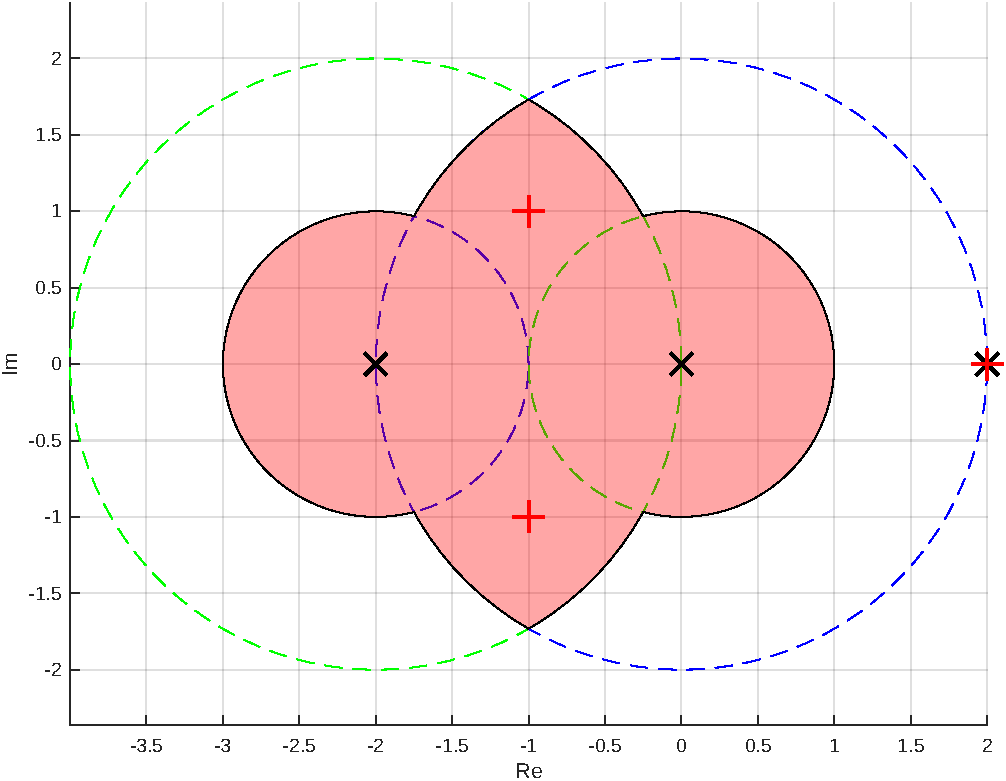
\includegraphics[width=\textwidth]{problems/problem_7_1.pdf}
    \caption{Gershgorin disks for $\matr{A}_1$. Black crosses mark disks' centres. Red crosses mark eigenvalues computed with the \MATLAB \texttt{eig} function. We may observe two features of the Gershgorin disks: (1) since $\matr{A}_1\in\mathfrak{R}$, any complex eigenvalues must occur in conjugate pairs (2) since the disk (point) with radius $r=0$ and centre in $(0,2)$ is disjoint from the other unions, it must be an eigenvalue}
    \label{fig:problem_7_1}
\end{figure}

\begin{figure}
    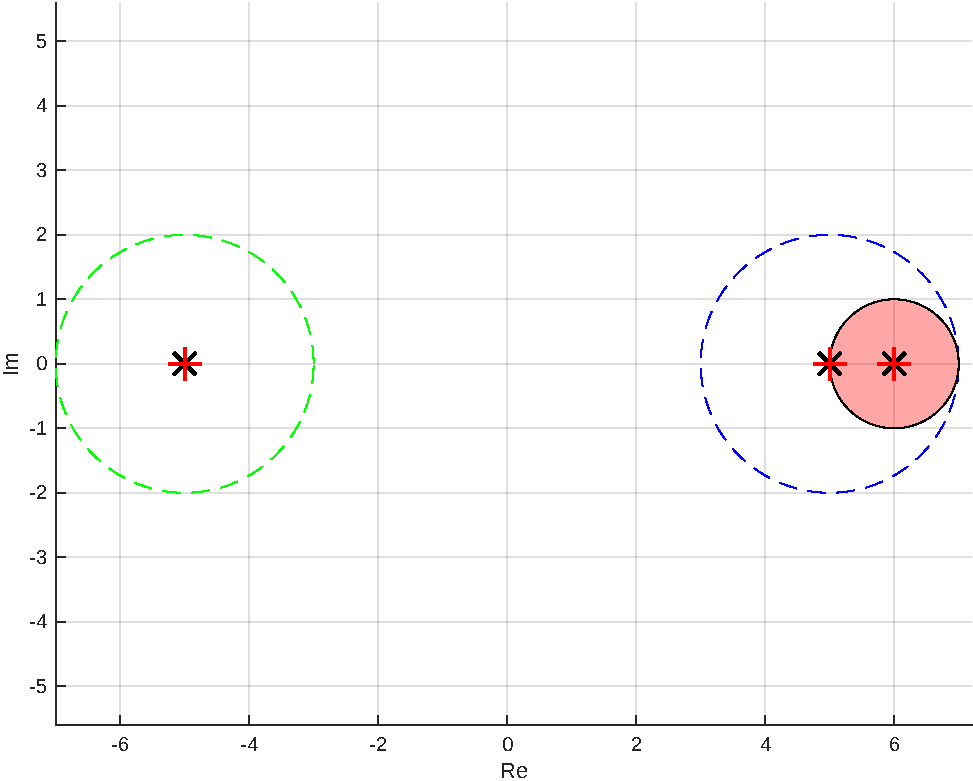
\includegraphics[width=\textwidth]{problems/problem_7_2.pdf}
    \caption{Gershgorin disks for $\matr{A}_2$. In such situation, the eigenvalue must lie in the point $(-5,0)$ and inside the red-coloured disk}
    \label{fig:problem_7_2}
\end{figure}

\begin{figure}
    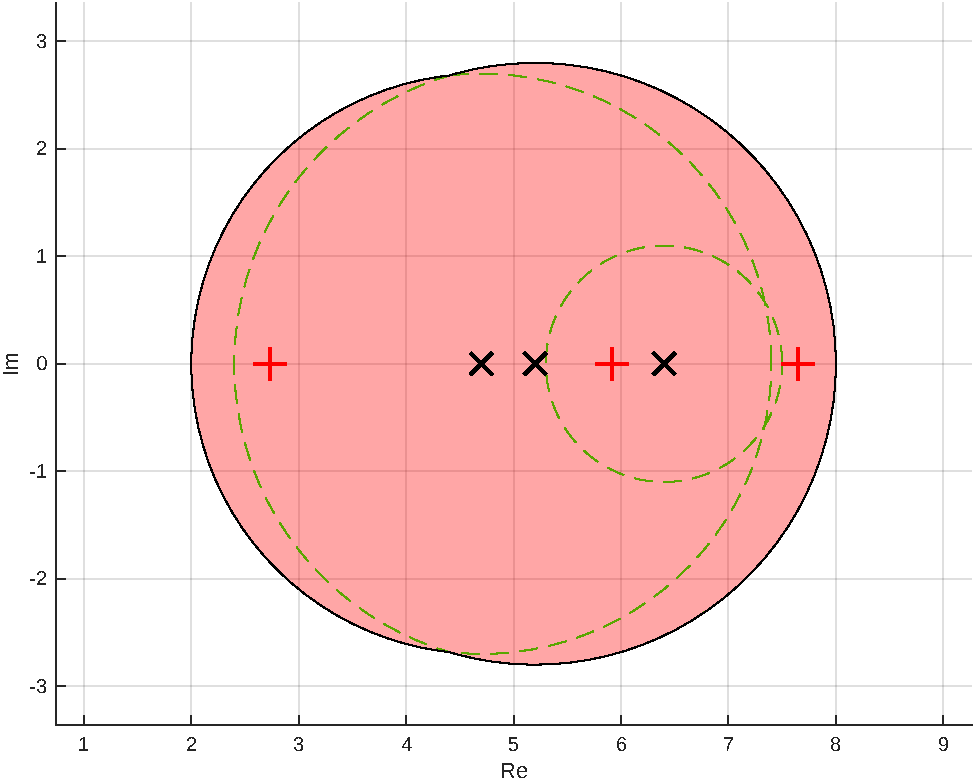
\includegraphics[width=\textwidth]{problems/problem_7_3.pdf}
    \caption{Gershgorin disks for $\matr{A}_3$. Since this matrix is not \textit{diagonally dominant}, the area bounding the eigenvalues is relatively is big}
    \label{fig:problem_7_3}
\end{figure}

% Since the the \textit{condition number} may be expressed as:
% \begin{equation*}
%     \kappa=\frac{\sigma_{\max}}{\sigma_{\min}}
% \end{equation*}
% and:
% \begin{equation*}
%     ||\mathbf{A}||_2=\max\sum_j|a_{ij}|
% \end{equation*}


% \begin{equation*}
%     \kappa(\mathbf{A})=||\mathbf{A}||_2\cdot||\mathbf{A}^{-1}||_2
% \end{equation*}
% Since the \textit{matrix norm} may be expressed as:
% \begin{equation*}
%     ||\mathbf{A}||=\max\sum_j|a_{ij}|
% \end{equation*}
% then the upper bound on the condition number is $\text{cond}(\matr{A}_1)=3\cdot2=6$.

% WHAT THE FUCK DO I HAVE TO DO TO ESTIMATE THE UPPER BOUND FOR THE CONDITION NUMBER XD WHICH ONE DXDYDZ
